% Short note on how the HOTEC x Frigidaire benchmark samples its problems and how its four algorithms work.
% Same layout as docs/scoring_note. Build: `make here` -> build/planning_note.pdf
\documentclass[10pt]{article}
\usepackage[a4paper,hmargin=1.7cm,vmargin=1.2cm]{geometry}
\usepackage{amsmath,amssymb,booktabs,enumitem}
\usepackage{graphicx}
\usepackage{tikz}
\usetikzlibrary{arrows.meta,decorations.pathmorphing,decorations.pathreplacing,shapes.geometric}
\setlist{itemsep=1pt,topsep=2pt,parsep=0pt}
\setlength{\parindent}{0pt}
\setlength{\parskip}{4pt}
\setlength{\emergencystretch}{1em}
\pagestyle{empty}

\newcommand{\vect}[1]{\mathbf{#1}}
\newcommand{\Cat}{\mathcal{C}}
\newcommand{\Obj}{\mathcal{O}}
\newcommand{\Buf}{\mathcal{B}}
\newcommand{\ind}{\mathbb{I}}
\newcommand{\free}{\operatorname{free}}
\newcommand{\legal}{\lambda}
\newcommand{\Slow}{S_{\mathrm{low}}}
\newcommand{\head}[1]{\par\smallskip\textbf{#1}\quad}
% a figure inside a step of Section 2: centered at its natural size, caption below
\newcommand{\mathfig}[3]{\par\smallskip{\centering #2\\[2pt]
  \parbox{0.92\linewidth}{\footnotesize\textbf{Fig.~#1.} #3}\par}\medskip}

\begin{document}
\setlength{\abovedisplayskip}{4pt}\setlength{\belowdisplayskip}{4pt}
\setlength{\abovedisplayshortskip}{2pt}\setlength{\belowdisplayshortskip}{2pt}

{\LARGE\bfseries How the benchmark samples and plans}\\[3pt]
{\small Start sampling, the pose catalogue, the goal, and the four algorithms \,\textperiodcentered\, HOTEC $\times$ Frigidaire benchmark \,\textperiodcentered\, 2026-09-30}

\medskip
\textbf{In one sentence:} only the start is drawn at random; every load (the goal, first-fit's, MCTS's) is a choice of one pose per dish from the same fixed catalogue under the same load rules, and the four algorithms differ in how they choose and in how they order the one-dish teleports that build it.
Track~A (greedy, RRT-Connect) must reach the given goal; track~B (first-fit, MCTS) picks its own load and is judged by its settled score $S$.

\section*{1\quad The idea}
\begin{enumerate}
\item \textbf{Start (random).} Draw how many dishes start on the counter, which ones, and where: random drops into the racks, messy stacks on the counter. Isaac builds the scene one dish at a time and keeps it only if it rests, reproduces, and can be cleared top-down.
\item \textbf{Catalogue (fixed).} Every dish kind has a fixed grid of rack poses (tine gap, lean, tilt, offset, lift). Poses that hit the closed appliance or the rack on its way in are removed once. A \emph{load} gives every dish one catalogue pose (or lets a rack dish stay where it is), with one dish per slot, no nested bowls, at least 3\,mm between dishes.
\item \textbf{Goal (track A).} Start from a first-fit load and move one dish at a time to the free pose that raises $S$ most; Isaac then builds that load and its settled poses become the goal.
\item \textbf{Greedy.} Send home any dish whose goal is free; if none, park one blocker on the counter. Planned on the collision mirror, then replayed.
\item \textbf{RRT-Connect.} Grow one tree of arrangements from the start and one from the goal, each edge one legal teleport, until they meet.
\item \textbf{First-fit (track B).} Give each dish, in roster order, the first free catalogue pose; then order the moves with the greedy sequencer.
\item \textbf{MCTS (track B).} Search over moves ``put this dish on this pose for good'', judging each partial plan by completing it to a full load and scoring that load.
\end{enumerate}

\small
\setlength{\abovedisplayskip}{3pt}\setlength{\belowdisplayskip}{3pt}
\section*{2\quad The math}
Each block below gives the math of the step with the same number in Section~1.
Figs.~1, 2, 3, 6 and 7b use the benchmark's own records (2026-09-29 run, 12 instances); Figs.~4, 5 and 7a are schematics.

\head{Notation.}
An instance has a roster $\Obj$ of $m$ dishes ($m=7$ easy, $15$ medium, $23$ hard), each of kind $\kappa(o)\in\{\text{plate},\text{bowl},\text{cup}\}$.
An \emph{arrangement} $X=(T_o)_{o\in\Obj}$ gives every dish a pose $T_o$ (a $4\times4$ rigid transform in world coordinates); $X_0$ is the settled start.
The counter slab carries a grid $\Buf$ of 14 parking cells ($7\times2$, pitch 0.25\,m), and at most $C$ dishes may be on the counter at once.
Everything an algorithm does is a sequence of \emph{moves} $(o,T)$: dish $o$ is teleported to $T$ and Isaac settles it (150\,+\,60 ticks at 120\,Hz).
Before a move is executed it must be \emph{legal} on the collision mirror (an FCL copy of the scene):
\begin{equation}
\begin{aligned}
\legal(X,o,T)={}&\ind\bigl[\text{$o$ at $T$ is FCL-clear of the appliance, the slab and every $o'\neq o$ at $T_{o'}$}\bigr]\\
&\cdot\ind\bigl[\text{no unmoved counter dish rests on $o$}\bigr]\cdot\ind\bigl[\text{order}(o,T)\bigr]\cdot\ind\bigl[\text{cap}(X,o,T)\bigr].
\end{aligned}
\label{eq:legal}
\end{equation}
$\text{order}(o,T)$ holds unless $T$ is $o$'s goal and a dish $o$ leans on in the certified build is not yet at its own goal; $\text{cap}(X,o,T)$ holds unless $T$ is on the counter, $T_o$ is not, and $C$ dishes are already there.
At a certified goal pose the appliance test and the test against dishes resting at their own goals are skipped (certified goal poses may touch; Isaac's settle is the judge).
The episode driver refuses an illegal command (non-fatal, counted; 25 refusals in a row abort the episode).

\head{Step 1: Start.}
With seed $\varsigma$ and tier slack $\sigma$ ($3$ easy, $2$ medium, $1$ hard), the number of counter dishes and the counter cap are
\begin{equation}
n\sim\mathcal{U}\bigl\{\lceil m/4\rceil,\dots,\lfloor 3m/4\rfloor\bigr\},\qquad C=n+\sigma,
\end{equation}
where $\mathcal{U}$ is the uniform distribution and $n$ depends on (tier, $\varsigma$) only.
Every other draw comes from the random stream of (tier, $\varsigma$, attempt $a$), so a rejected attempt is re-rolled as $a+1$ with fresh draws:
\begin{itemize}
\item the counter set $\Obj_{\mathrm c}\subset\Obj$, a uniform $n$-subset; the rest are rack dishes: plates in the lower rack, bowls and cups in either rack with probability $\tfrac12$;
\item a rack drop: rotation $R\sim\mathcal{U}(SO(3))$, bounding-box centre uniform in the rack box (9\,cm in from its walls, 2--6\,cm above its floor), then lifted in 1\,cm steps (up to 16\,cm) until FCL-clear of everything already settled; up to 1500 draws per dish;
\item the counter stacks: per kind, the dishes are shuffled and cut into stacks of height $h\sim\mathcal{U}\{1,\dots,\min(4,\text{dishes left})\}$ (cups always $h=1$), a bowl or cup stack face-down with probability $\tfrac12$; each dish gets a yaw $\psi\sim\mathcal{U}[0,2\pi)$ and a tilt $\tau\sim\mathcal{U}[0,4^\circ]$ about a random horizontal axis; a stack base lies uniformly in a box of twice the summed base footprint (aspect 1.6, every rim 2\,cm inside the slab), and each higher dish is offset from it uniformly within a 15\,mm disc.
\end{itemize}
Each dish settles 1\,s before the next is dropped.
The attempt is kept only if (i) the scene rests (contact depth under 2\,mm over 5\,s), (ii) exactly $n$ dishes are on the counter and the rest in the racks, (iii) it reproduces within 10\,mm\,/\,15$^\circ$ when teleported back, and (iv) a top-down clearing order exists in Isaac in which no removal moves a remaining dish more than 10\,mm\,/\,20$^\circ$.

\mathfig{1}{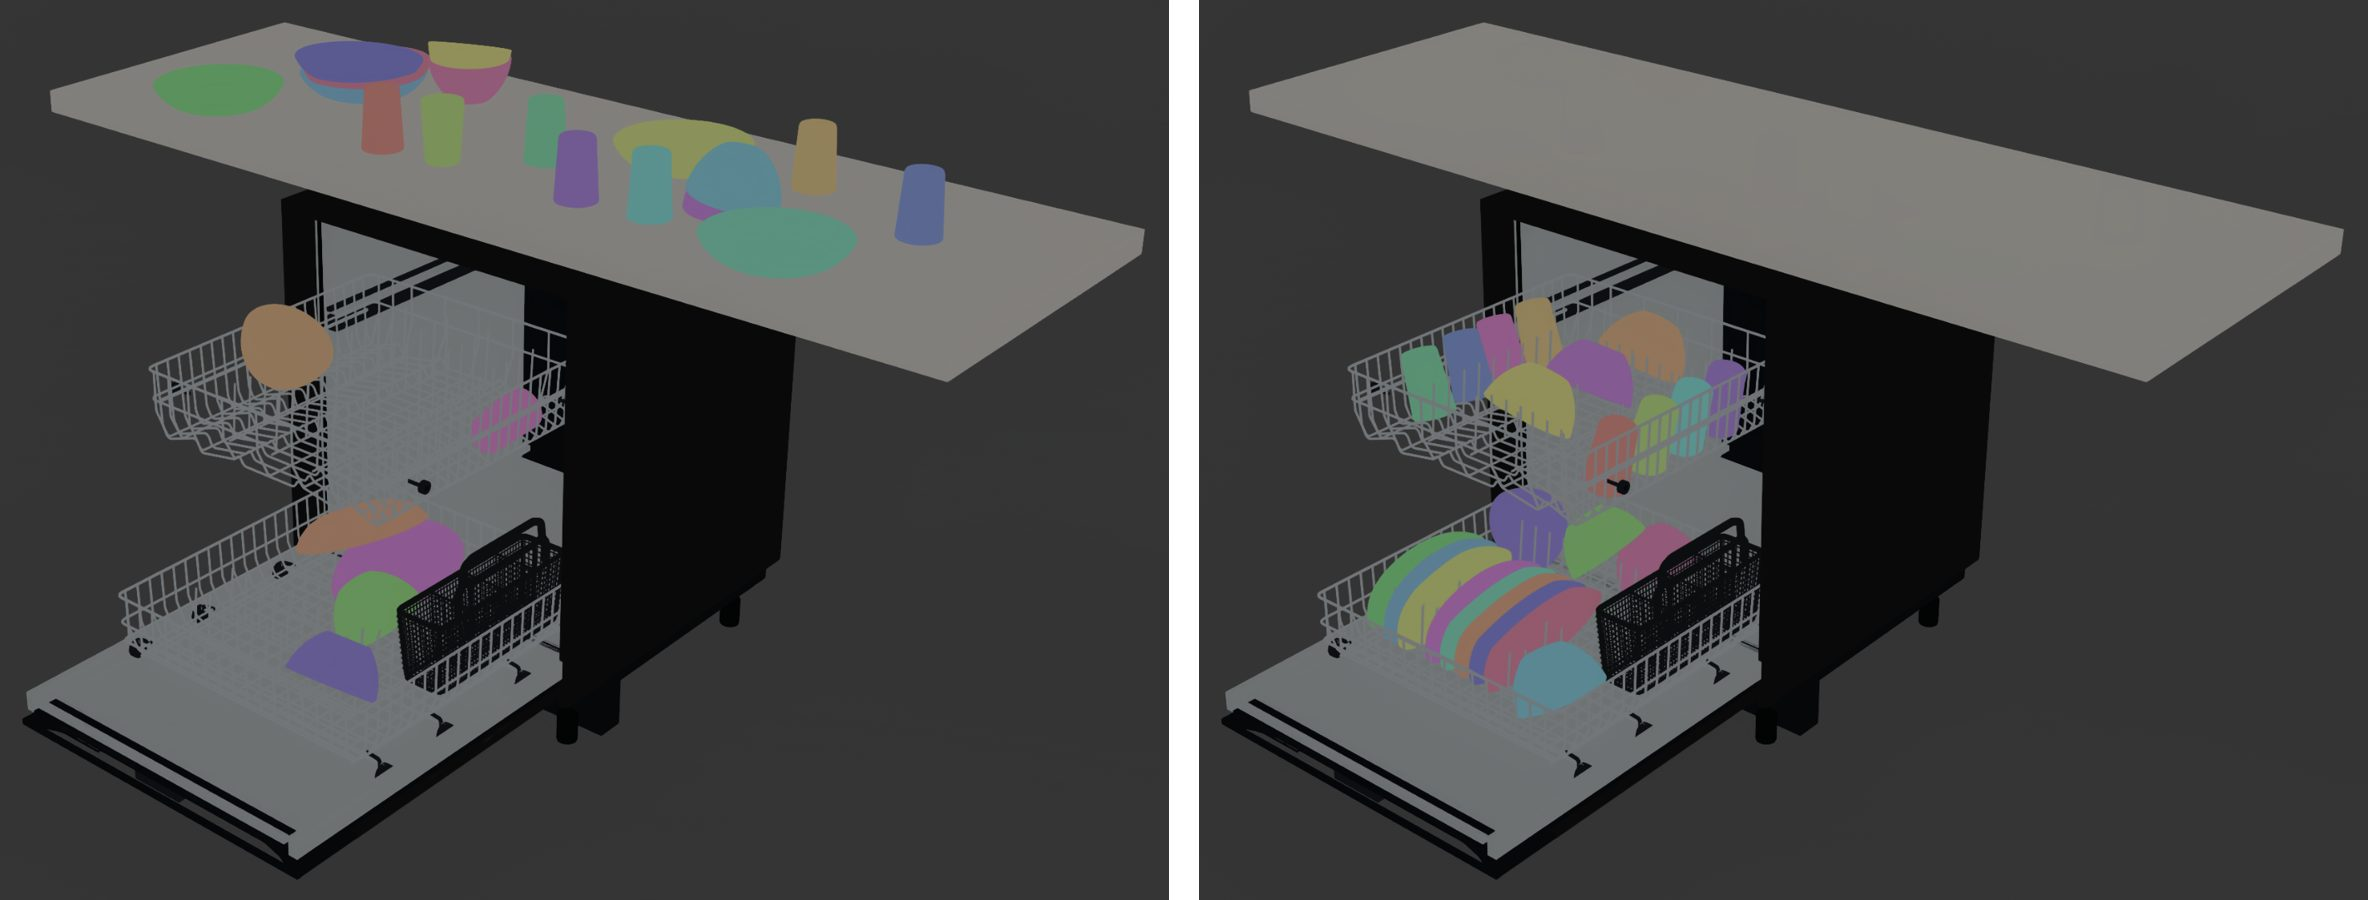
\includegraphics[width=0.94\linewidth]{figures/fig_stills.jpg}}
{Steps 1 and 3 on hard\_s0 ($m=23$). Left: the sampled start $X_0$, $n=17$ dishes in 13 stacks on the counter ($C=18$), 6 dropped into the racks. Right: the goal $G$ of track~A, the settled Isaac build of the goal search's load ($S_{\mathrm{ref}}=0.173$).}

\head{Step 2: Catalogue and load rules.}
The catalogue $\Cat_\kappa$ is a finite product grid of rack-local poses, built once and identical for every instance and every algorithm:
plates: bank $\times$ tine gap $\times$ lean $\{-32,-28,\dots,-12\}^\circ$ $\times$ sideways offset $\{-12,-10,\dots,12\}$\,mm;
bowls: zone $\times$ 8 tilt families ($105,120,135,150^\circ$ about $x$ or $y$) $\times$ row offset $\times$ $x$ on a 5\,mm grid $\times$ lift $\{0,20,40,60\}$\,mm, plus front-right and upper-rack variants;
cups: 12 upper-rack slots $\times$ 4 (offset, lean, lift) variants.
The \emph{usable} catalogue keeps the poses that pass the benchmark's filters (no mid-zone bowl, front-right bowls at $x\le0.165$\,m, inside the tub walls), clear the closed appliance, and clear the cabinet at all 25 positions of the rack's slide in:
\begin{equation}
\Cat^\star_\kappa=\{c\in\Cat_\kappa:\ \text{filters}(c)\wedge\text{clear}(c)\wedge\text{sweep}(c)\},\qquad
|\Cat^\star_{\mathrm{plate}}|=180,\ |\Cat^\star_{\mathrm{bowl}}|=1814,\ |\Cat^\star_{\mathrm{cup}}|=24
\end{equation}
(of 1482, 14\,742 and 48).
A rack dish that starts tub-clear, not pooling and not resting on another dish also has a \emph{keep} pose $k_o$: its start pose, 2\,mm higher.
A \emph{load} $L$ maps every dish to a pose, $L(o)\in\Cat^\star_{\kappa(o)}\cup\{k_o\}$.
Given the poses $L(o')$ already assigned to other dishes, the poses still \emph{free} for $o$ are
\begin{equation}
\begin{aligned}
\free(o\mid L)=\bigl\{c\in\Cat^\star_{\kappa(o)}:\ {}&\text{for every assigned } o'\neq o\text{: (R1) a different slot (plates, cups), (R2) not nested (bowls),}\\
&\text{(R3) } \operatorname{dist}(c,L(o'))\ge\delta,\ \text{(R4) neither $c$ nor the pair $(c,L(o'))$ banned}\bigr\},
\end{aligned}
\end{equation}
with $\operatorname{dist}$ the FCL distance between the two dishes' collision pieces and $\delta=3$\,mm.
Bans are poses or pose pairs that failed an Isaac build before; they apply to every later search.
A load is \emph{valid} if every $L(o)$ is free given the others, and \emph{feasible} if no dish in it pools; $S(L)$ is the scoring note's load score of its commanded poses.

\mathfig{2}{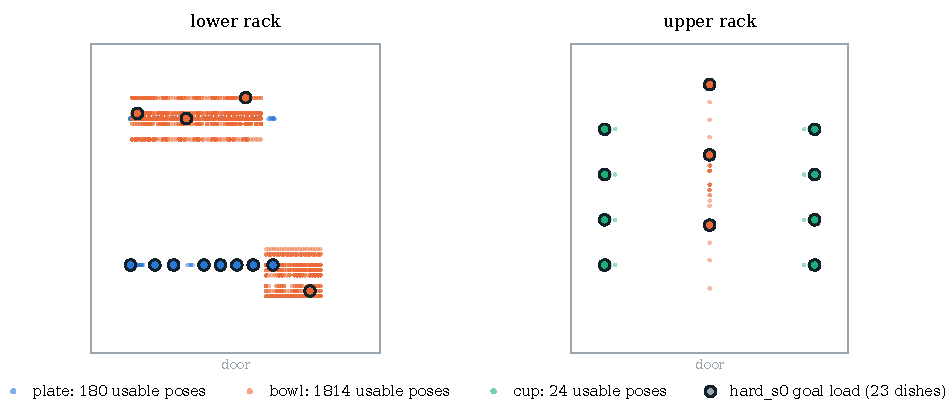
\includegraphics{figures/fig_catalogue.pdf}}
{Step 2 in symbols, top view of the two racks (rack-local $x$ across, $y$ from the door to the back; dish origins). Light dots: the 2018 usable poses $\Cat^\star_\kappa$ (many share one $(x,y)$ and differ in lean, tilt or lift). Large dots: the 23 poses of the hard\_s0 goal load, one per dish, all taken from these dots.}

\head{Step 3: Goal (track A).}
The goal search starts from a valid load $L_0$: on attempt $0$ the keeps and then first-fit (Step~6); on a re-roll a first-fit with the catalogue order shuffled (up to 20 tries); failing both, an earlier Isaac-validated goal of the same tier.
It then runs \emph{coordinate ascent}, at most 2 sweeps over the roster.
For dish $o$ with current load $L$, let $A_o=\free(o\mid L)\cup\{k_o\}$ and let $E^{\mathrm{iso}}(c)$ be the dish's exposure at pose $c$ alone in the empty racks (200 dots, 32 spray points).
The tried set is the 6 poses of $A_o$ with the highest $E^{\mathrm{iso}}$ plus 2 drawn uniformly from $A_o$ (the only random draws of the goal search), and
\begin{equation}
c^\ast=\operatorname*{arg\,max}_{c\in\text{tried}} S\bigl(L[o\mapsto c]\bigr),\qquad
L\leftarrow L[o\mapsto c^\ast]\quad\text{if } L[o\mapsto c^\ast]\text{ is feasible and } S\bigl(L[o\mapsto c^\ast]\bigr)>S(L)+10^{-4},
\end{equation}
where $L[o\mapsto c]$ is $L$ with dish $o$ moved to $c$ and $S$ is evaluated at full resolution (500 dots, 64 spray points).
It stops after a sweep without gain or after 2 sweeps; it has no time limit (178\,s on hard\_s0).
Isaac then checks the load in one joint settle and builds it one dish at a time; the settled poses $G=(g_o)$, each commanded 3\,mm high, are the goal, and $S_{\mathrm{ref}}=S$ of the settled poses.
Each dish a placed dish leans on in that build gives an order constraint (used in~\eqref{eq:legal}).
The instance is kept only if the greedy sequencer of Step~6 can reach $G$ from $X_0$ under the cap $C$.
A dish is \emph{at goal} when it is within 15\,mm laterally, 20\,mm vertically and 15$^\circ$ of tilt of $g_o$ (plates 18\,mm\,/\,20\,mm\,/\,16$^\circ$); the lower bound on the move count is the number of counter dishes plus the rack dishes that $G$ does not keep.

\mathfig{3}{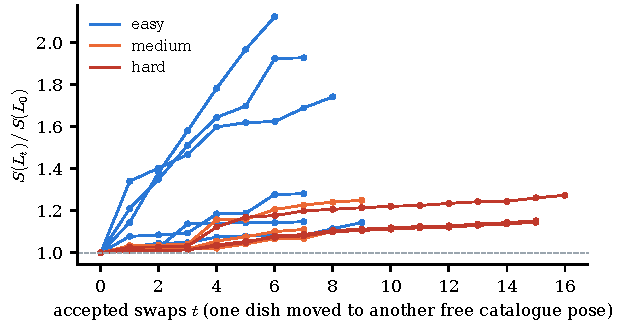
\includegraphics{figures/fig_ascent.pdf}}
{Step 3 in symbols: $S(L_t)/S(L_0)$ over the accepted swaps $t$ of the goal search of all 12 instances. On easy (7 bowls, free space) the ascent raises the first-fit score by 14--112\,\%, in the full medium and hard racks by 11--27\,\%.}

\head{Step 4: Greedy (track A).}
With $G$ fixed and the roster in file order, one call of the greedy rule on arrangement $X$ returns
\begin{equation}
\begin{aligned}
&\text{pass 1: } (o,g_o)\ \text{for the first $o$ not at goal with } \legal(X,o,g_o)=1;\\
&\text{pass 2: } (b,\beta)\ \text{with } \beta=\text{the first cell of } \Buf \text{ with } \legal(X,b,\beta)=1,
\end{aligned}
\end{equation}
where pass 2 runs only if pass 1 found nothing and fewer than $C$ dishes are on the counter, and $b$ is the first blocker of the first not-at-goal dish $o$ (a dish in the way of $(o,g_o)$, or one $o$ must wait for) that is not at its goal and has not been parked since it last reached its goal; a dish blocked by the appliance or the slab is skipped.
If neither pass finds a move, the rule gives up.
\emph{greedy\_offline} runs this rule to completion on the mirror before the first move (each planned move lands exactly, at-goal means exactly at $g_o$; at most $10m$ moves and $0.95$ of the 60\,s budget), then replays the list blind; it replans from the observed arrangement only when a dish settles more than 6\,cm from where it was sent.
Nothing in it is random, and it never looks at $S$.

\mathfig{4}{% Fig. 4: the greedy rule on a two-dish example. Dish o waits on the counter; its goal g_o is occupied by dish b,
% which sits at a non-goal pose in the rack. Pass 1 fails for o, pass 2 parks b, pass 1 then sends o and b home.
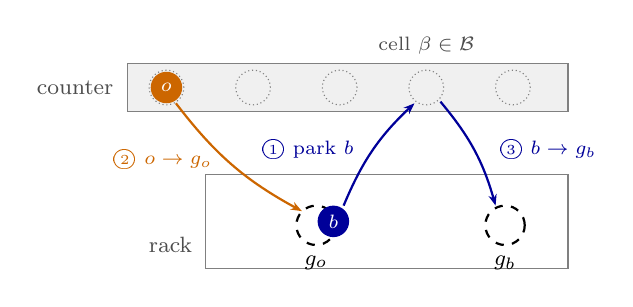
\begin{tikzpicture}[x=1cm,y=1cm,>={Stealth[length=4pt]},font=\footnotesize]
  % counter slab with its parking cells
  \fill[gray!12] (0,2.0) rectangle (5.6,2.6);
  \draw[gray] (0,2.0) rectangle (5.6,2.6);
  \node[anchor=east,gray!60!black] at (-0.05,2.3) {counter};
  \foreach \x in {0.5,1.6,2.7,3.8,4.9} \draw[gray,densely dotted] (\x,2.3) circle (0.22);
  \node[anchor=south,gray!60!black,font=\scriptsize] at (3.8,2.6) {cell $\beta\in\mathcal{B}$};
  % rack with the two goal poses
  \draw[gray] (1.0,0) rectangle (5.6,1.2);
  \node[anchor=east,gray!60!black] at (0.95,0.3) {rack};
  \draw[dashed,thick] (2.4,0.55) circle (0.25);
  \node[anchor=north] at (2.4,0.29) {$g_o$};
  \draw[dashed,thick] (4.8,0.55) circle (0.25);
  \node[anchor=north] at (4.8,0.29) {$g_b$};
  % the dishes now
  \fill[orange!80!black] (0.5,2.3) circle (0.2);
  \node[white,font=\scriptsize\bfseries] at (0.5,2.3) {$o$};
  \fill[blue!60!black] (2.62,0.6) circle (0.2);
  \node[white,font=\scriptsize\bfseries] at (2.62,0.6) {$b$};
  % the three moves, labels placed clear of the arrows
  \draw[->,thick,blue!60!black] (2.75,0.8) to[bend left=12] (3.65,2.1);
  \node[anchor=east,blue!60!black,font=\scriptsize] at (3.0,1.5) {\textcircled{\tiny 1} park $b$};
  \draw[->,thick,orange!80!black] (0.62,2.1) to[bend right=12] (2.22,0.73);
  \node[anchor=east,orange!80!black,font=\scriptsize] at (1.2,1.35) {\textcircled{\tiny 2} $o\to g_o$};
  \draw[->,thick,blue!60!black] (3.98,2.12) to[bend left=12] (4.68,0.8);
  \node[anchor=west,blue!60!black,font=\scriptsize] at (4.6,1.5) {\textcircled{\tiny 3} $b\to g_b$};
\end{tikzpicture}
}
{Step 4 in symbols. Dish $o$ (counter) cannot go home because $b$ sits on $g_o$, so pass~1 fails; pass~2 parks the blocker $b$ on a free cell $\beta\in\Buf$ (move~1); pass~1 then sends $o$ home (move~2) and later $b$ (move~3). With the counter full, pass~2 is skipped and the rule gives up: medium\_s1 and s2 stopped at moves 6 and 11.}

\head{Step 5: RRT-Connect (track A).}
A node of a tree is an arrangement (a commanded pose per dish), an edge one legal teleport of one dish.
In this benchmark every dish's candidate poses are the goals of its kind plus the counter cells,
\begin{equation}
\mathcal{P}_\kappa=\{g_{o'}:\kappa(o')=\kappa\}\cup\Buf,
\end{equation}
so a dish that leaves its start pose never returns to it.
A sample $\tilde X$ is the goal $G$ with probability $0.3$, else every dish draws its pose independently and uniformly from $\mathcal{P}_{\kappa(o)}$.
The distance between two arrangements counts the dishes at different poses, $d(X,Y)=\sum_o\ind[T_o\neq T'_o]$ (poses equal within 0.1\,mm).
One \emph{extend} of tree $\mathcal{T}$ toward $\tilde X$ takes $X_{\mathrm{near}}=\arg\min_{X\in\mathcal{T}}d(X,\tilde X)$, draws up to 4 of the dishes where they differ in random order, and adds the first child $X_{\mathrm{near}}[o\mapsto\tilde T_o]$ whose move is legal and whose arrangement is new (positions on a 1\,mm grid).
Two trees grow, $\mathcal{T}_a$ from $X_0$ and $\mathcal{T}_b$ from $G$; each iteration extends one tree toward a sample, then extends the other toward the new node $X_{\mathrm{new}}$ again and again (\emph{connect}) until an extend fails or reaches it, and the two trees swap roles.
The goal tree is checked backwards: its edge $Y\to Y[o\mapsto T]$ is kept only if the reverse move, from $Y[o\mapsto T]$ back to $T_o$ of $Y$, is legal, because that is the move the plan will execute.
When the trees meet, the plan is the start tree's path to the meeting node followed by the goal tree's path replayed in reverse.
The search uses 0.95 of the 60\,s budget (and at most 200\,000 iterations), then replays its plan blind, replanning only when a dish settles more than 6\,cm off.

\mathfig{5}{% Fig. 5: RRT-Connect in arrangement space. Every node is a whole arrangement (one pose per dish), every edge
% one legal teleport of one dish. Left tree from the start X_0, right tree from the goal G; one extend toward a
% sample (X_new lies on the way from X_near to the sample), then the other tree's connect steps toward X_new.
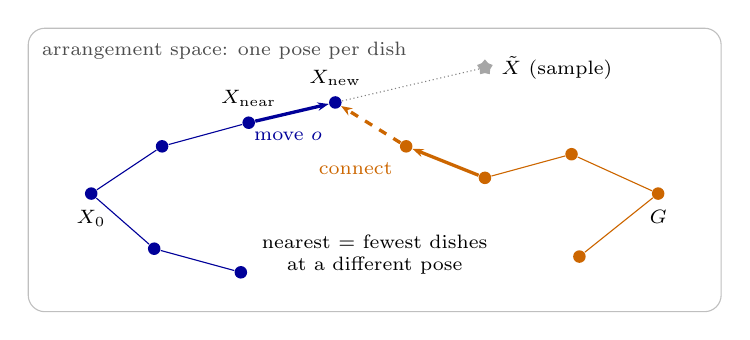
\begin{tikzpicture}[x=1cm,y=1cm,>={Stealth[length=4pt]},font=\footnotesize,
                    n/.style={circle,fill=#1,inner sep=1.6pt}]
  \draw[gray!50,rounded corners=6pt] (-0.2,-0.1) rectangle (8.6,3.5);
  \node[anchor=north west,gray!60!black,font=\scriptsize] at (-0.15,3.45) {arrangement space: one pose per dish};
  % start tree
  \node[n=blue!60!black,label={[font=\scriptsize]below:$X_0$}] (a0) at (0.6,1.4) {};
  \node[n=blue!60!black] (a1) at (1.4,0.7) {};
  \node[n=blue!60!black] (a2) at (1.5,2.0) {};
  \node[n=blue!60!black,label={[font=\scriptsize]above:$X_{\rm near}$}] (a3) at (2.6,2.3) {};
  \node[n=blue!60!black] (a4) at (2.5,0.4) {};
  \draw[blue!60!black] (a0)--(a1) (a0)--(a2) (a2)--(a3) (a1)--(a4);
  % sample and the extend step
  \node[star,star points=5,fill=gray!70,inner sep=1.4pt,label={[font=\scriptsize]right:$\tilde X$ (sample)}] (s) at (5.6,3.0) {};
  \draw[gray,densely dotted] (a3)--(s);
  \node[n=blue!60!black,label={[font=\scriptsize]above:$X_{\rm new}$}] (an) at (3.7,2.557) {};
  \draw[blue!60!black,very thick,->] (a3)--(an);
  \node[anchor=north,blue!60!black,font=\scriptsize] at (3.1,2.3) {move $o$};
  % goal tree
  \node[n=orange!80!black,label={[font=\scriptsize]below:$G$}] (b0) at (7.8,1.4) {};
  \node[n=orange!80!black] (b1) at (6.8,0.6) {};
  \node[n=orange!80!black] (b2) at (6.7,1.9) {};
  \node[n=orange!80!black] (b3) at (5.6,1.6) {};
  \draw[orange!80!black] (b0)--(b1) (b0)--(b2) (b2)--(b3);
  % connect steps of the goal tree toward X_new
  \node[n=orange!80!black] (c1) at (4.6,2.0) {};
  \draw[orange!80!black,very thick,->] (b3)--(c1);
  \draw[orange!80!black,very thick,->,dashed] (c1)--(an);
  \node[anchor=north east,orange!80!black,font=\scriptsize] at (4.55,1.92) {connect};
  \node[anchor=north,font=\scriptsize,align=center] at (4.2,1.0) {nearest = fewest dishes\\ at a different pose};
\end{tikzpicture}
}
{Step 5 in symbols. A sample $\tilde X$ (star) pulls the start tree (blue) from its nearest node $X_{\mathrm{near}}$ by one move to $X_{\mathrm{new}}$; the goal tree (orange) then extends toward $X_{\mathrm{new}}$ until it reaches it. Measured: 16--33 extends on easy, 2382--20\,021 on medium/hard; hard\_s1 spent 57\,s and 10\,004 nodes without meeting.}

\head{Step 6: First-fit (track B).}
With the roster $o_1,\dots,o_m$ in file order (plates, bowls, cups) and $\Cat^\star_\kappa$ in its fixed catalogue order, first-fit assigns
\begin{equation}
L(o_i)=\text{the first } c\in\Cat^\star_{\kappa(o_i)} \text{ with } c\in\free\bigl(o_i\mid L(o_1),\dots,L(o_{i-1})\bigr),
\end{equation}
and fails if some dish has no free pose. It uses no keeps, no ranking and no score, and no random draw on the first attempt.
The \emph{greedy sequencer} then orders the moves to $L$: Step~4's rule with the counter dishes first (top of a stack first), dishes that still carry another never moved, and blockers parked only while fewer than $C$ dishes are on the counter.
Isaac builds the load one dish at a time (each dish lands within 8\,cm with contact depth under 2\,mm, no placed dish moves more than 10\,mm\,/\,20$^\circ$); the built poses become the targets, the moves are re-sequenced under the build's order and replayed.
A failed build bans the pose or pair it blamed and re-plans, up to 6 attempts; a re-plan is the same first-fit under the new bans, and a few seeded shuffles of the catalogue order only when that no longer packs or repeats an earlier load.

\mathfig{6}{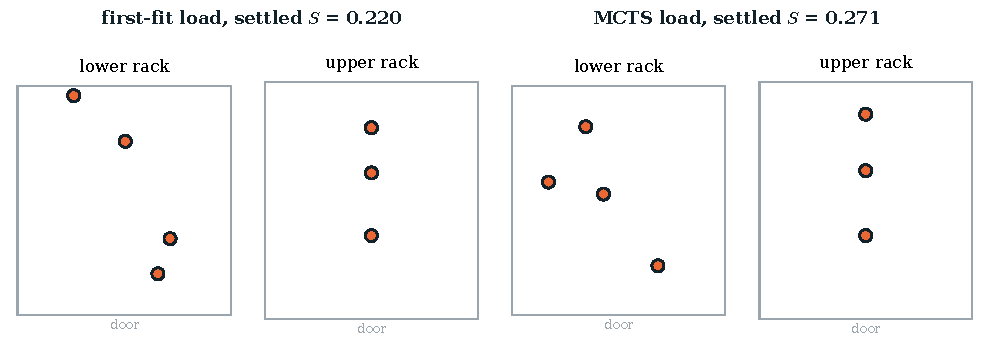
\includegraphics{figures/fig_loads.pdf}}
{Steps 6 and 7 on easy\_s0 (7 bowls; top view, dish origins): first-fit takes the first free poses of the catalogue, MCTS keeps the high-exposure ones that still leave room for the others. Settled $S$ against $S_{\mathrm{ref}}=0.288$ of the track-A goal.}

\head{Step 7: MCTS (track B).}
A search state is $s=(X,K)$: the arrangement on the mirror and the set $K\subseteq\Obj$ of dishes already \emph{committed} to their final pose; the root is $(X_0,\emptyset)$ and $s$ is terminal when $K=\Obj$.
The moves out of $s$, for an uncommitted dish $o\notin K$, are
\begin{equation}
\text{place}(o,c),\ c\in\free(o\mid L_K);\qquad \text{keep}(o)=\text{place}(o,k_o);\qquad \text{buffer}(o,\beta),\ \beta\in\Buf,
\end{equation}
where $L_K$ holds the committed poses, place and keep add $o$ to $K$, buffer parks a not-yet-parked dish without committing it, and every move must satisfy~\eqref{eq:legal}.
Placements are capped at 6 per dish: its 3 poses with the highest $E^{\mathrm{iso}}$ in the whole catalogue that are free, then poses from a \emph{pool} of complete packings (first-fit plus up to 12 seeded shuffles of its order, built in the first $\le$15\,s; the shuffles are the search's only random draws).
Children are generated lazily in this order (placements round-robin over the dishes in sequencing order, keeps after each dish's placements, parks last).
Each node stores its visit count $N(s)$ and value sum $W(s)$; one \emph{simulation} has four steps:
\begin{enumerate}
\item \textbf{Select.} From the root, while $s$ has as many children as progressive widening allows, $|\text{children}(s)|\ge 2\,N(s)^{1/2}$, go to
\begin{equation}
s\leftarrow\operatorname*{arg\,max}_{s'\in\text{children}(s)}\ \frac{W(s')/N(s')-v_{\min}}{v_{\max}-v_{\min}}+c\,\sqrt{\frac{\ln N(s)}{N(s')}},\qquad c=1/\sqrt2,
\label{eq:uct}
\end{equation}
with $v_{\min},v_{\max}$ the smallest and largest rollout value seen so far; the first term favours children that have paid off, the second children rarely tried.
\item \textbf{Expand.} Add the next legal move of $s$ as a new child $s'$.
\item \textbf{Roll out.} Complete $s'$ to a full load $L(s')$: take its parent's completed load, put the moved dish at its new pose, and re-place only the uncommitted dishes it now clashes with (its vacated pose first, then first-fit, restarting with the failing dish first, up to 9 times). The value is
\begin{equation}
V(s')=\begin{cases}\Slow\bigl(L(s')\bigr)&\text{if the completion succeeds and no dish pools},\\ 0&\text{otherwise,}\end{cases}
\end{equation}
with $\Slow$ the load score at low resolution (120 dots, 32 spray points). A pose whose repair fails is never offered again; values are cached by the set of committed poses.
\item \textbf{Back up.} Every node on the path gets $N\leftarrow N+1$ and $W\leftarrow W+V(s')$.
\end{enumerate}
The root starts at the best pooled packing. After 55\,s (of the 60\,s budget) the answer is the best complete load any rollout found (ties: fewer tree moves): the tree's moves to that node, then the greedy sequencer for the remaining dishes; it is re-scored at full resolution and goes through the same Isaac build as first-fit's.

\mathfig{7}{\begin{tabular}{@{}c@{\hspace{6mm}}c@{}}\raisebox{4mm}{% Fig. 7 (a): one MCTS simulation. Nodes are (arrangement, committed set); the thick path is the UCT descent, the
% dashed child the one expansion, the wavy arrow the rollout (local repair to a complete load), the grey arrows the
% back-up of its value to every node on the path.
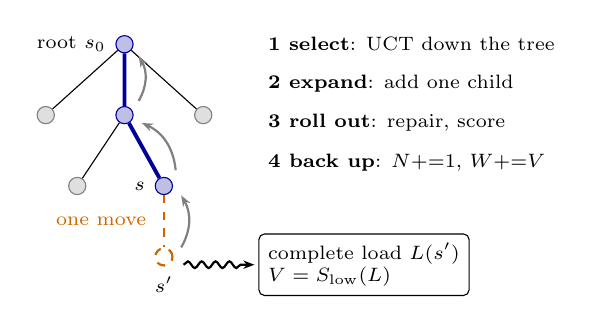
\begin{tikzpicture}[x=1cm,y=1cm,>={Stealth[length=4pt]},font=\footnotesize,
                    n/.style={circle,draw=#1,fill=#1!25,inner sep=2.2pt}]
  \node[n=blue!60!black,label={[font=\scriptsize]left:root $s_0$}] (r) at (1.6,3.2) {};
  \node[n=gray] (c1) at (0.6,2.3) {};
  \node[n=blue!60!black] (c2) at (1.6,2.3) {};
  \node[n=gray] (c3) at (2.6,2.3) {};
  \node[n=gray] (d1) at (1.0,1.4) {};
  \node[n=blue!60!black,label={[font=\scriptsize]left:$s$}] (d2) at (2.1,1.4) {};
  \node[circle,draw=orange!80!black,dashed,thick,inner sep=2.2pt,label={[font=\scriptsize]below:$s'$}] (e) at (2.1,0.5) {};
  \draw (r)--(c1) (r)--(c3) (c2)--(d1);
  \draw[blue!60!black,line width=1.4pt] (r)--(c2) (c2)--(d2);
  \draw[orange!80!black,dashed,thick] (d2)--(e);
  \node[anchor=east,orange!80!black,font=\scriptsize] at (2.0,0.95) {one move};
  % back-up, beside the path
  \draw[->,gray,thick] (2.32,0.62) to[bend right=30] (2.32,1.28);
  \draw[->,gray,thick] (2.25,1.6) to[bend right=30] (1.82,2.2);
  \draw[->,gray,thick] (1.78,2.48) to[bend right=30] (1.78,3.05);
  % rollout to a complete load
  \draw[->,decorate,decoration={snake,amplitude=1.2pt,segment length=5pt,post length=3pt},thick] (2.35,0.4) -- (3.25,0.4);
  \node[draw,rounded corners=2pt,font=\scriptsize,align=left,anchor=west] at (3.3,0.4) {complete load $L(s')$\\ $V=S_{\rm low}(L)$};
  % step labels
  \node[anchor=west,font=\scriptsize] at (3.3,3.2) {\textbf{1 select}: UCT down the tree};
  \node[anchor=west,font=\scriptsize] at (3.3,2.7) {\textbf{2 expand}: add one child};
  \node[anchor=west,font=\scriptsize] at (3.3,2.2) {\textbf{3 roll out}: repair, score};
  \node[anchor=west,font=\scriptsize] at (3.3,1.7) {\textbf{4 back up}: $N{+}{=}1$, $W{+}{=}V$};
\end{tikzpicture}
} & 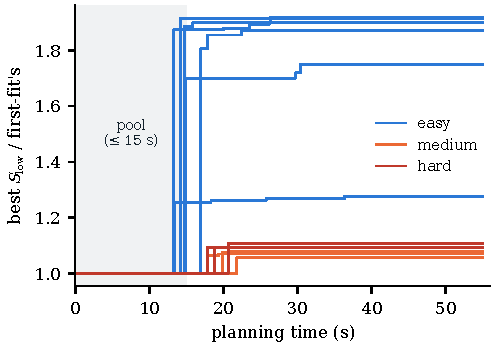
\includegraphics{figures/fig_mcts.pdf}\\ {\footnotesize (a) one simulation} & {\footnotesize (b) best $\Slow$ found, all 12 first attempts}\end{tabular}}
{Step 7 in symbols. (a) The selected path (thick), the new child $s'$ (dashed), its rollout to a complete load and the back-up of $V$. (b) The pool (grey band) already gives most of the gain over first-fit (up to $1.9\times$ on easy); the tree then adds 0--4\,\%. 94--304 simulations per attempt, trees at most 3 moves deep.}

\head{Same catalogue, different choices.}
\begin{center}\footnotesize
\begin{tabular}{@{}lllp{3.9cm}p{7.3cm}@{}}
\toprule
& track & uses $S$ & random draws & result (easy / medium / hard)\\
\midrule
goal search & -- & full res. & 2 alternatives per dish; shuffles on re-rolls & defines $G$ and $S_{\mathrm{ref}}$ (no time limit)\\
greedy\_offline & A & no & none & solved 6/6, 1/3, 3/3 in 7.8, 20.0, 28.3 moves\\
RRT-Connect & A & no & samples, extend order & solved 6/6, 2/3, 2/3 in 8.3, 33.0, 52.5 moves\\
first-fit & B & no & none (shuffles on re-plans) & solved 5/6, 3/3, 2/3 at $S/S_{\mathrm{ref}}$ 0.666, 0.975, 0.964\\
MCTS & B & low res. & pool shuffles & solved 6/6, 3/3, 3/3 at $S/S_{\mathrm{ref}}$ 1.036, 1.019, 1.008\\
\bottomrule
\end{tabular}
\end{center}
Track-A lower bounds are 7, 15 and 23 moves. The goal search runs without a budget while track~B plans within 60\,s per attempt, so $S/S_{\mathrm{ref}}$ is not an equal-budget comparison.

\head{Parameters.}
Counter slab $1.8\times0.6$\,m, top at $z=0.914$\,m, 14 cells; cap $C=n+3,\,n+2,\,n+1$; settle per move 150\,+\,60 ticks at 120\,Hz; refusal and settle loops abort at 25; goal hover 3\,mm, keep hover 2\,mm; load clearance $\delta=3$\,mm; goal ascent: 2 sweeps, top 6 + 2 random, gain $>10^{-4}$; RRT-Connect: goal bias 0.3, 4 dishes per extend, 0.95 of the budget; MCTS: 6 placements per dish (3 ranked + 3 pooled), pool $\le12$ packings in $\le15$\,s, $c=1/\sqrt2$, widening $2N^{1/2}$, 9 repair restarts, rollout $\Slow$ at 120 dots $\times$ 32 points, 5\,s reserve; planning budget 60\,s per episode (track~B: per attempt, up to 6 attempts).

{\footnotesize Coordinates: world frame, metres, $z$ up; rack-local poses in each rack's frame ($x$ across, $y$ from the door to the back). Results: \texttt{frigidaire/docs/hotec\_bench.md} (2026-09-29 run). Source: start sampling \texttt{start} in \texttt{frigidaire\_bench\_kit.py}; catalogue \texttt{candidate\_families} in \texttt{frigidaire\_hotec\_exposure\_search.py}, filters, load rules, \texttt{first\_fit}, \texttt{goal\_search} and \texttt{make\_bench\_world} in \texttt{frigidaire\_bench.py}; greedy \texttt{Greedy}/\texttt{OfflineGreedy} in \texttt{src/dishsim/rearrange.py}; \texttt{RRTConnect} in \texttt{src/dishsim/rrt.py}; the greedy sequencer \texttt{sequence} in \texttt{planner.py}; MCTS in \texttt{mcts.py} (both \texttt{frigidaire/src/dishsim\_frigidaire/}).\par}

\end{document}
